%% AMS-LaTeX Created by Wolfram Mathematica 9.0 : www.wolfram.com

\documentclass{article}
\usepackage{amsmath, amssymb, graphics, setspace}

\newcommand{\mathsym}[1]{{}}
\newcommand{\unicode}[1]{{}}

\newcounter{mathematicapage}
\begin{document}

\title{Pregunta 1}
\author{}
\date{}
\maketitle

Definimos las funciones a utilizar en el problema:

\begin{doublespace}
\noindent\(\pmb{\text{Clear}[\text{s1},\text{s2},\text{s3},F,x,y,z,l,m,n,t,\text{surfacePlot},\text{vectorPlot}];}\\
\pmb{\text{s1}=x^2+y^2+z^2-2^2;}\\
\pmb{\text{s2}=z+2;}\\
\pmb{\text{s3}=x^2+y^2-z-1;}\\
\pmb{F=\left\{x^3,y^3,z^3\right\};}\)
\end{doublespace}

Graficamos las superficies intersectadas junto con el campo vectorial dado:

\begin{doublespace}
\noindent\(\pmb{\text{surfacePlot} = \text{ContourPlot3D}[\{\text{s1},\text{s2},\text{s3}\},\{x,-4,4\},\{y,-4,4\},}\\
\pmb{\{z,-4,4\},\text{Contours}\to \{0\},}\\
\pmb{\text{ContourStyle}\to \text{Directive}[\text{Orange},\text{Opacity}[0.5],\text{Specularity}[\text{White},30]],}\\
\pmb{\text{Mesh}\to \text{None},}\\
\pmb{\text{BoundaryStyle}\to \{1\to \text{None},2\to \text{None},3\to \text{None},\{1,3\}\to \{\{\text{Blue},\text{Tube}[.05]\}\},}\\
\pmb{\{1,2\}\to \{\{\text{Blue},\text{Tube}[.05]\}\}\},\text{ImageSize}\to \{300,300\},}\\
\pmb{\text{AxesLabel}\to \{X,Y,Z\},\text{ViewPoint}\to \{1,4,2\}];}\\
\pmb{\text{vectorPlot} = \text{VectorPlot3D}[F,\{x,-4,4\},\{y,-4,4\},\{z,-4,4\},}\\
\pmb{\text{VectorColorFunction}\to \text{{``}DeepSeaColors{''}}];}\\
\pmb{\text{Show}[\text{surfacePlot},\text{vectorPlot}]}\)
\end{doublespace}

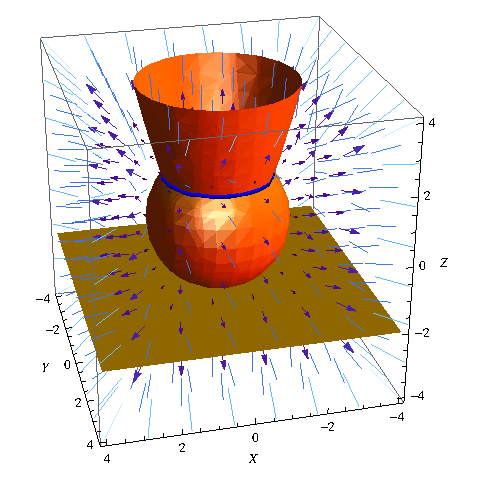
\includegraphics{lab3_gr1.eps}

Parametrizaremos las curvas respecto a coordenadas esf{\' e}ricas:

\begin{doublespace}
\noindent\(\pmb{t=\{x,y,z\};}\\
\pmb{x=2\text{Cos}[\theta ]\text{Sin}[\phi ];}\\
\pmb{y=2\text{Sin}[\theta ]\text{Sin}[\phi ];}\\
\pmb{z=2\text{Cos}[\phi ];}\)
\end{doublespace}

Calculamos el vector normal de la superficie:

\begin{doublespace}
\noindent\(\pmb{\text{Needs}[\text{{``}VectorAnalysis$\grave{ }${''}}]}\\
\pmb{n=\text{CrossProduct}\left[\partial _{\theta }t,\partial _{\phi }t\right]\text{//}\text{FullSimplify} ;}\\
\pmb{\text{(* Podemos omitir el signo negativo resultante *)}}\\
\pmb{n=n*-1; }\\
\pmb{n}\)
\end{doublespace}

\begin{doublespace}
\noindent\(\left\{4 \text{Cos}[\theta ] \text{Sin}[\phi ]^2,4 \text{Sin}[\theta ] \text{Sin}[\phi ]^2,2 \text{Sin}[2 \phi ]\right\}\)
\end{doublespace}

Luego, el campo vectorial queda como:

\begin{doublespace}
\noindent\(\pmb{F \text{//}\text{FullSimplify}}\)
\end{doublespace}

\begin{doublespace}
\noindent\(\left\{8 \text{Cos}[\theta ]^3 \text{Sin}[\phi ]^3,8 \text{Sin}[\theta ]^3 \text{Sin}[\phi ]^3,8 \text{Cos}[\phi ]^3\right\}\)
\end{doublespace}

Observando la grafica, notamos que el barrido del parametro $\theta $ es de 0 a 2$\pi $, mientras que $\phi $, hace un recorrido desde la intersecci{\'
o}n hasta $\pi $. Luego, el valor de esa intersecci{\' o}n es:

\begin{doublespace}
\noindent\(\pmb{\text{FindRoot}[\{\text{s1}-\text{s3}==0\}\text{/.}\text{Cos}[\phi ]\to l,\{l,0\}]}\\
\pmb{m=\text{ArcCos}[\text{{``}0.651388{''}}]}\)
\end{doublespace}

\begin{doublespace}
\noindent\(\{l\to 0.651388\}\)
\end{doublespace}

\begin{doublespace}
\noindent\(0.861384\)
\end{doublespace}

Finalmente, el flujo total que pasa por la superficie encerrada est{\' a} dada por la integral:

\begin{doublespace}
\noindent\(\pmb{\int _0^{2\pi }\int _m^{\pi }F.nd\phi d\theta }\)
\end{doublespace}

\begin{doublespace}
\noindent\(199.331\)
\end{doublespace}

\begin{doublespace}
\noindent\(\pmb{\text{Clear}[\text{edp},x,y,z,r,u,t,\theta ]}\)
\end{doublespace}

\begin{doublespace}
\noindent\(\{\{u[x,t]\to C[1][-t+x]+C[2][t+x]\}\}\)
\end{doublespace}

\end{document}
